\documentclass[]{article}

\usepackage[margin=1.0in]{geometry}
\usepackage{amsmath}
\usepackage{amsfonts}
\usepackage{amsthm}
\usepackage{graphicx}
\usepackage{amssymb}

\usepackage{mathtools}

%opening
\title{A Flare Domain Version of Hejhal's Algorithm: Dealing with Infinite Volume Fundamental Domains}
\author{Alex Karlovitz}
\date{}

\begin{document}
	
	\maketitle
	
Hejhal's algorithm in its original form fails to converge when the group in question has an infinite volume fundamental domain.
To rectify this, we utilize an expansion of a Maass form in polar coordinates in $\mathbb{H}$ after mapping the fundamental domain over to a domain containing ``flares.''
These notes discuss the details of this process.

\section*{What is a Flare?}

Most Fuchsian groups for $SL(2, \mathbb{R})$ contain an infinite number of hyperbolic elements.
Hyperbolic matrices are diagonalizable over $SL(2, \mathbb{R})$, and thus we may assume (perhaps after conjugation) that such a Fuchsian group contains a diagonal matrix, say
\[
A_\kappa =
\begin{pmatrix}
	\sqrt{\kappa} & 0 \\
	0 & 1/\sqrt{\kappa}
\end{pmatrix}
\]
for some $\kappa > 1$.
Note that the action of this matrix on $\mathbb{H}$ is $z \mapsto \kappa z$.
Thus, a fundamental domain for the action on $\mathbb{H}$ of \textit{this matrix only} is
$$
\{ z \in \mathbb{H} : 1 < |z| < \kappa \}
$$
When we add in the rest of the matrices of our Fuchsian group, there will exist a fundamental domain which is a subset of this half-ring.

Now assume that $\Gamma$ is a non-cocompact Fuchsian group containing the diagonal matrix $A_\kappa$.
Since a fundamental domain for $\Gamma$ has infinite volume, its boundary must contain an interval of positive measure on the real line (as opposed to simply a cusp).
Thus, it is plausible to expect a fundamental domain to have a subset of the form
$$
\{ z \in \mathbb{H} : 1 < |z| < k, 0 < \arg z < \alpha \}
$$
We refer to such a fundamental domain as a \textit{flare domain}, and we call the aforementioned subset a \textit{flare}.

\subsection*{Example: Hecke Triangle Groups}

Consider the Hecke triangle group
$$
\Gamma_r = \left\langle
	\begin{pmatrix}
		1 & 1 \\
		0 & 1
	\end{pmatrix},
	\begin{pmatrix}
		0 & -r \\
		1/r & 0
	\end{pmatrix}
	\right\rangle
$$
where $0 < r < 1/2$.
This group has a fundamental domain $\mathcal{F}_r := \{ z = x + iy : 0 < x < 1, |z| > r, |z - 1| > r \}$ (see Figure \ref{Fr}).
\begin{figure}[h]
	\centering
	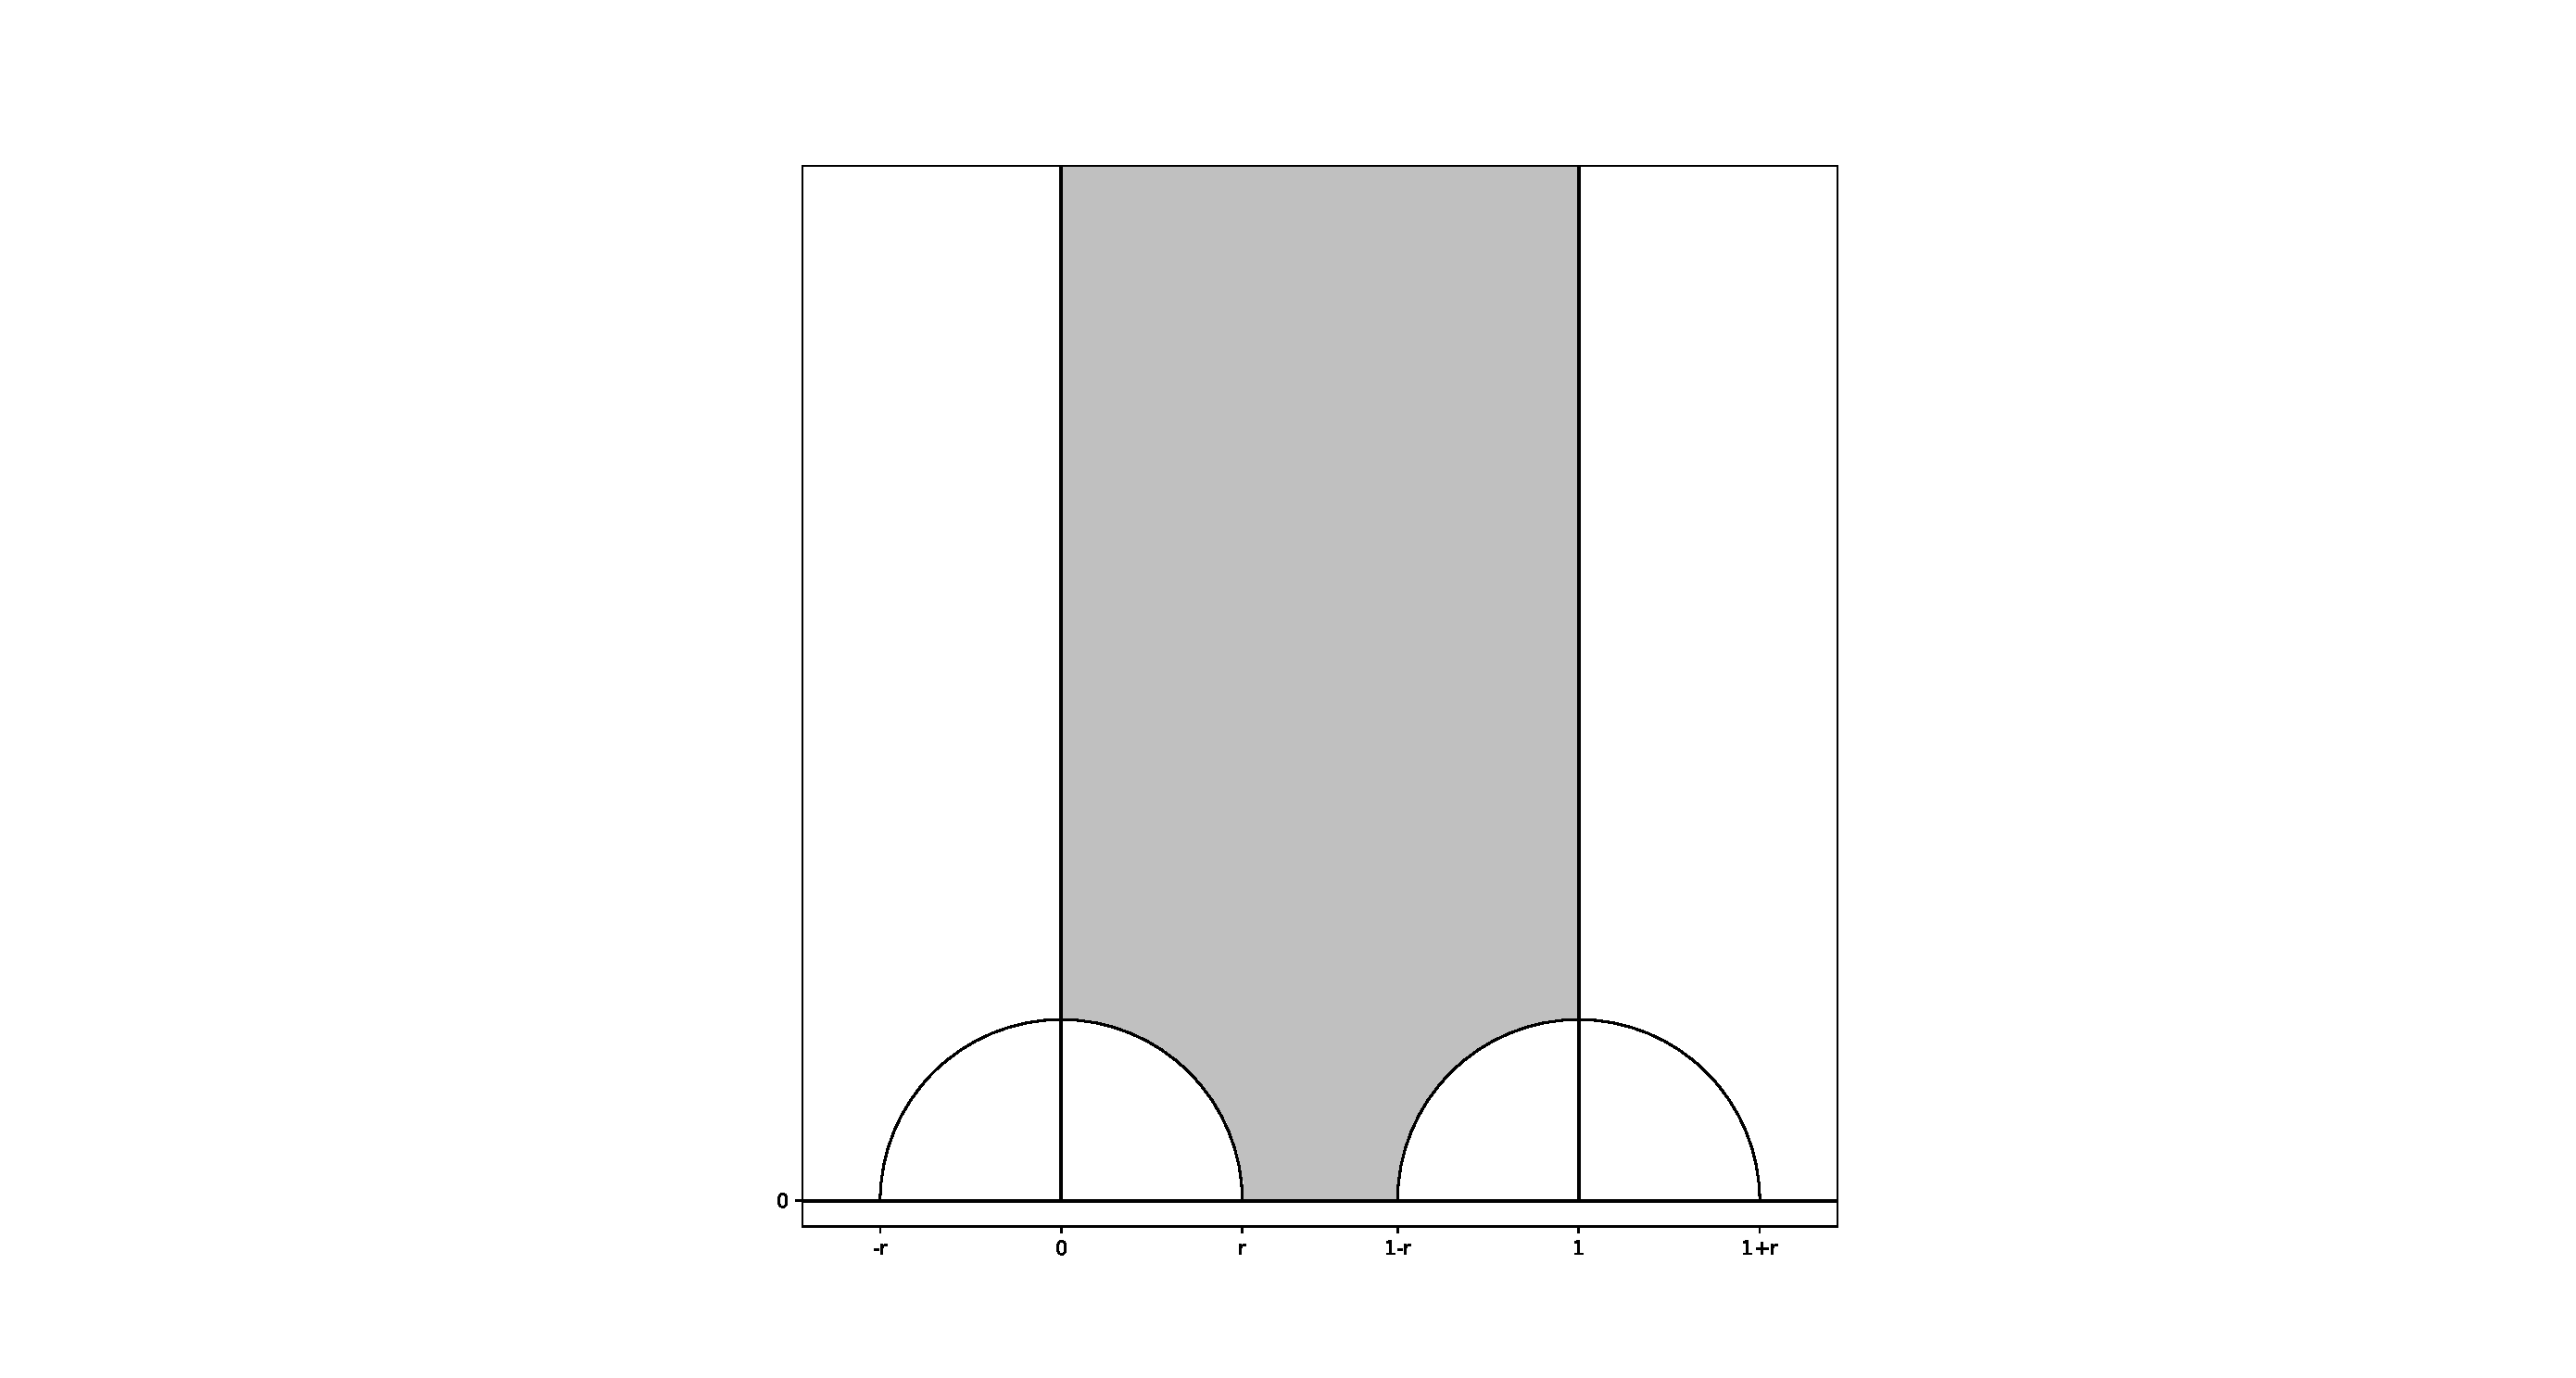
\includegraphics[trim=400 60 380 80, clip, width=0.6\linewidth]{gamma_r_fundl.pdf}
	\caption{$\mathcal{F}_r$ for $r = 7/20$}
	\label{Fr}
\end{figure}
We use this $\mathcal{F}_r$ instead of the standard fundamental domain centered at $0$ since it makes clear that we have exactly one flare (in addition to the one cusp).

Next, we find a hyperbolic matrix in $\Gamma_r$.
Looking at small words in the generators, one quickly finds
$$
A :=
\begin{pmatrix}
	1 & 1 \\
	0 & 1
\end{pmatrix}
\begin{pmatrix}
	0 & -r \\
	1/r & 0
\end{pmatrix} =
\begin{pmatrix}
	1/r & -r \\
	1/r & 0
\end{pmatrix}
$$
(Since $0 < r < 1/2$, we have that tr$(A) = 1/r > 2$, so $A$ is indeed hyperbolic).
We let $C$ be $A$'s axis, i.e., $C$ is the geodesic between the fixed points of $A$.
These points are
$$
z_1 = \frac{1 - \sqrt{1 - 4r^2}}{2} ~~ \text{and} ~~ z_2 = \frac{1 + \sqrt{1 - 4r^2}}{2}
$$
Note the following facts:
\begin{itemize}
	\item $z_1 < r < 1 - r < z_2$
	\item $C$ is orthogonal to $|z| = r$ and $|z - 1| = r$ (Kontorovich had a quick argument for this using some theorem from differential geometry, but of course we could always just verify the claim with calculus)
	\item $A$ maps $|z| = r$ to $|z - 1| = r$
\end{itemize}
For any $h > 0$, we also define the curve $C(h)$ to be the arc of the circle centered at $\frac{1}{2} - ih$ from $z_1$ to $z_2$.
See Figure \ref{FrWithCs} for a visual of these curves.
\begin{figure}[h]
	\centering
	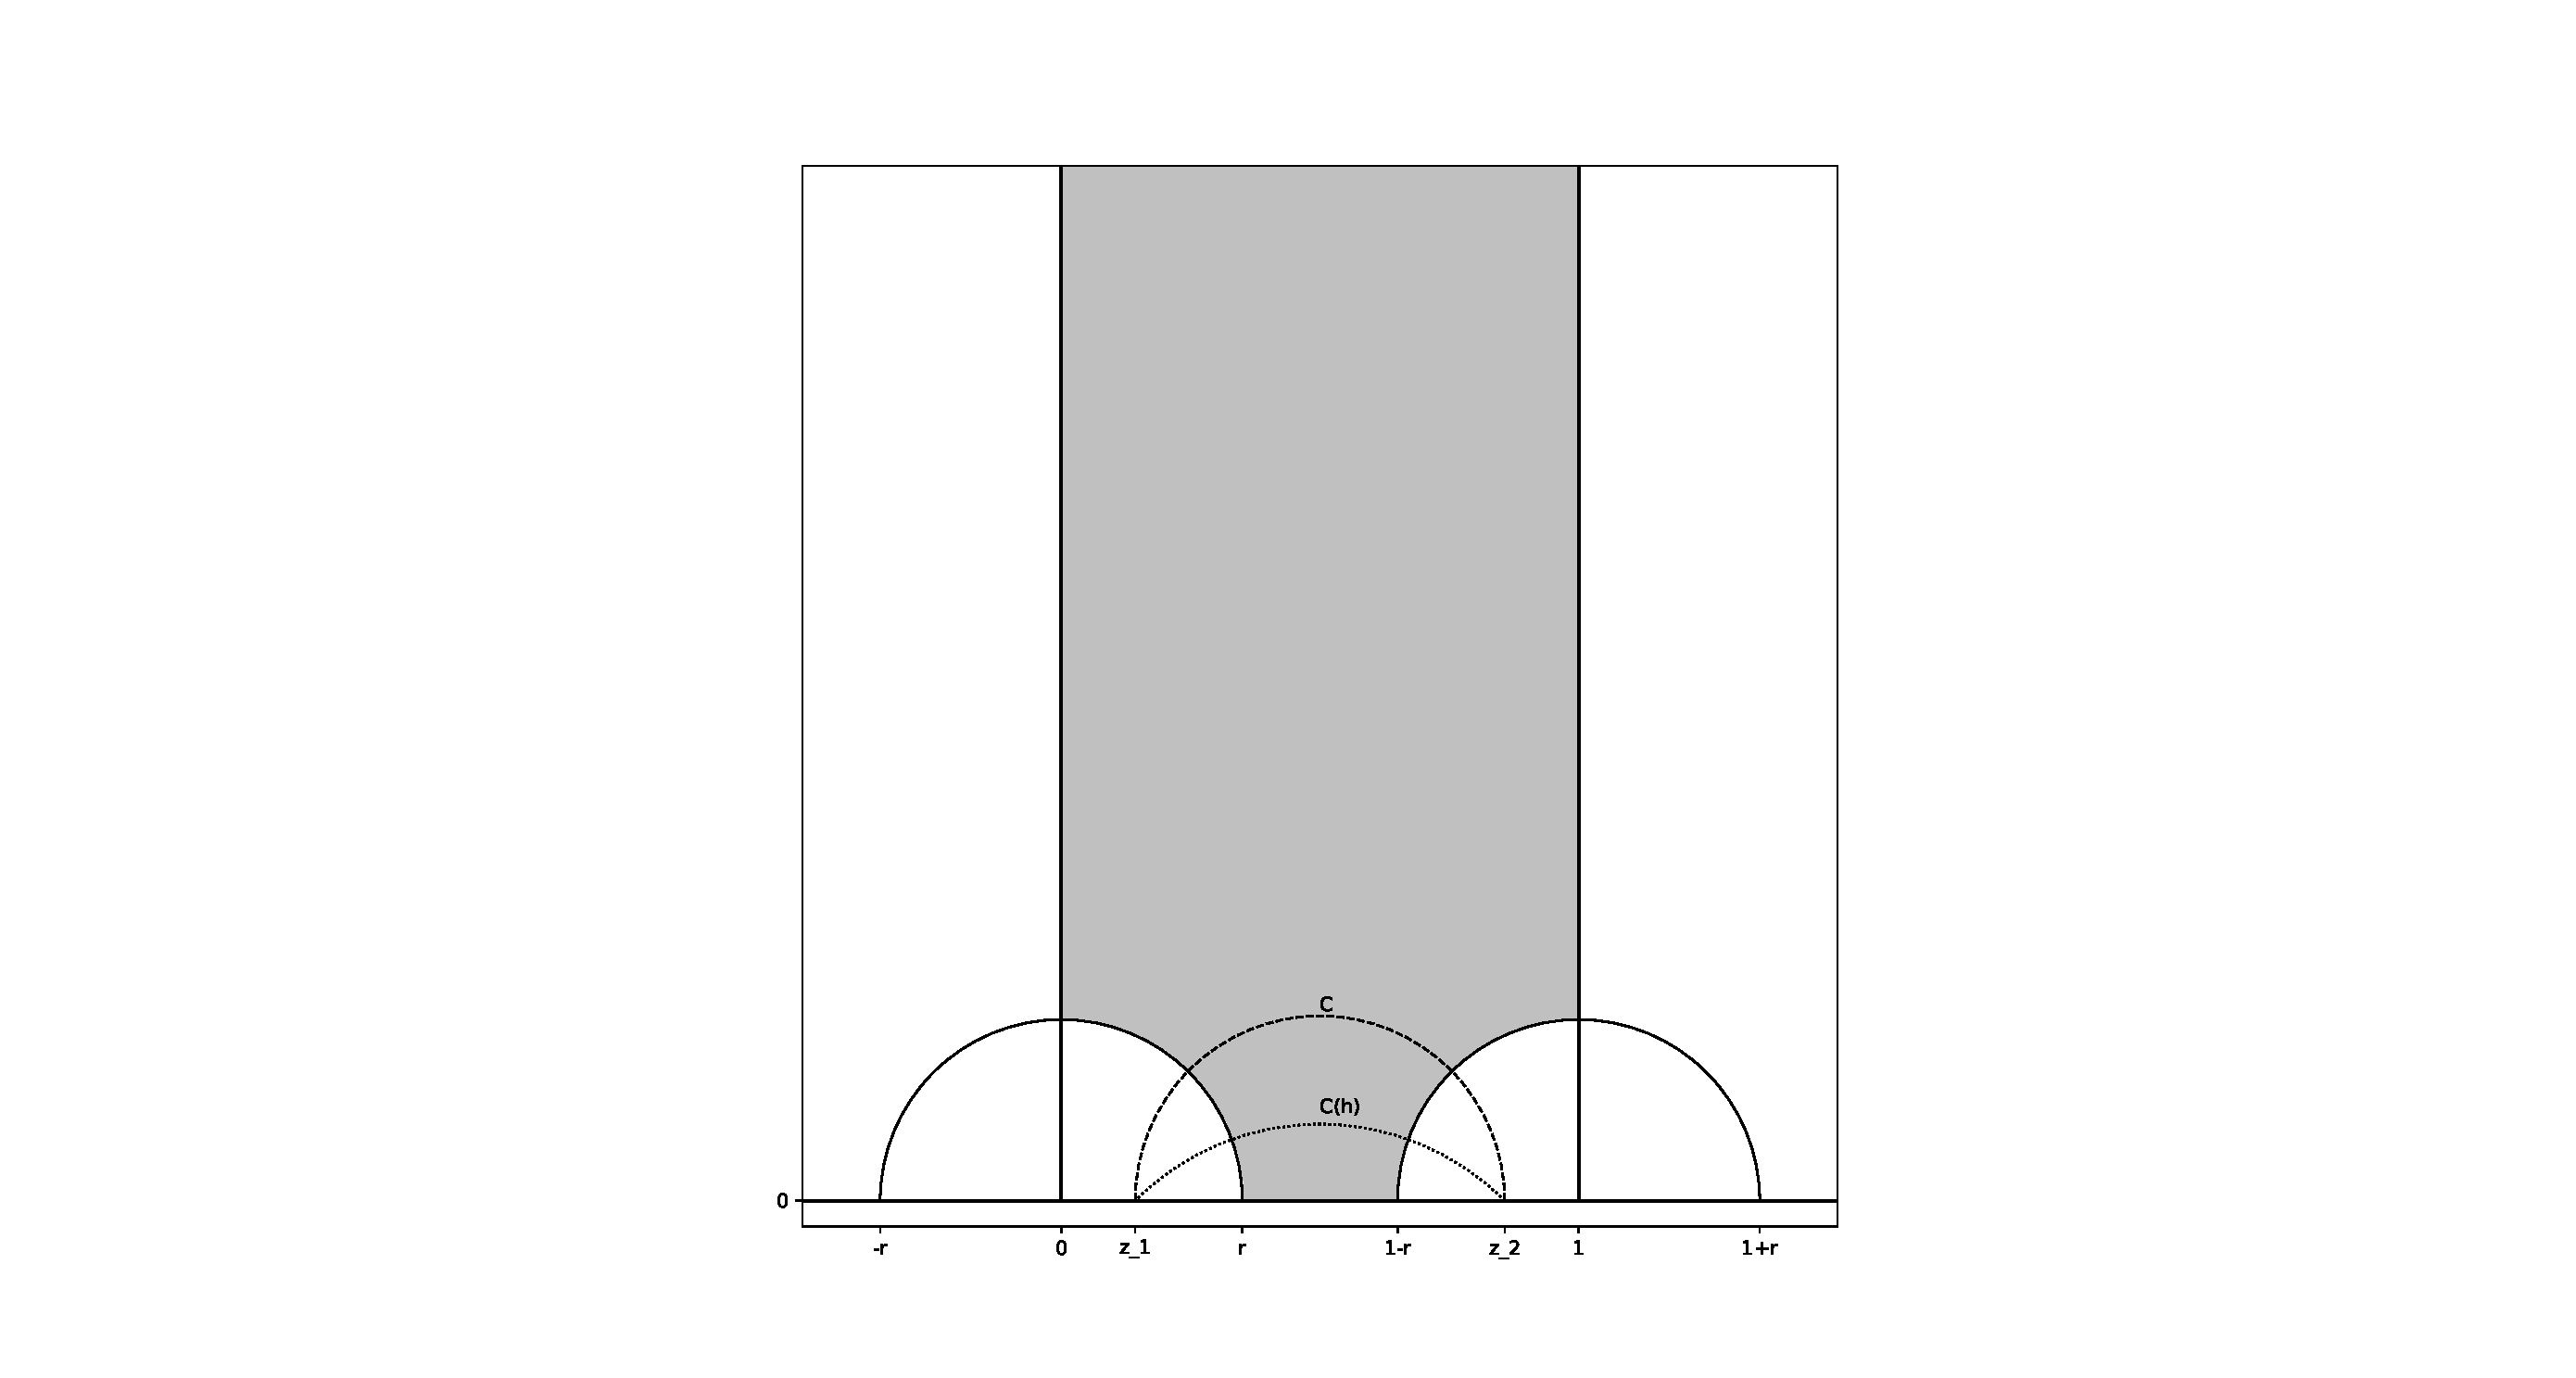
\includegraphics[trim=400 60 380 80, clip, width=0.6\linewidth]{F_r_with_Cs.pdf}
	\caption{$\mathcal{F}_r$ for $r = 7/20$ with $C$ and $C(h)$ for some $h > 0$}
	\label{FrWithCs}
\end{figure}
Note that the portion of $\mathcal{F}_r$ which lies above $C(h)$ has finite volume.
After conjugation, it is the area of $\mathcal{F}_r$ that lies \textit{below} $C(h)$ which will become a flare.
Using classical geometry, it can also be shown that the acute angle $C(h)$ makes with the real axis is
$$
\alpha = \frac{\pi}{2} - \arctan\left( \frac{h}{\sqrt{\frac{1}{4} - r^2}} \right)
$$
Note that if we have a specific value of $\alpha$ in mind, it would be straightforward to solve for $h > 0$ in this equation.

Next, we let $U$ be the matrix whose action on $\mathbb{H}$ is
$$
U(z) = c\frac{z - z_1}{z - z_2} ~~~~~ \left( c := \frac{r - z_2}{r - z_1} \right)
$$
$U$ is chosen so that $U(z_1) = 0$ and $U(z_2) = \infty$.
The scaling constant $c$ is chosen so that $U(r) = 1$.

\textbf{Claim}: $UAU^{-1}$ is diagonal.
To verify the claim, first note that $UAU^{-1}(\infty) = \infty$.
The elements of $SL(2, \mathbb{R})$ which stabilize infinity have bottom-left entry equal to $0$, so we conclude that $UAU^{-1}$ has the form
$\begin{psmallmatrix}
	a & b \\
	0 & d
\end{psmallmatrix}$
where $ad = 1$.
Next, note that $UAU^{-1}(0) = 0$.
Since we also have that $UAU^{-1}(0) = b/d$, we conclude that $b = 0$.
So this matrix is diagonal, as claimed.

Thus far, we have found a hyperbolic matrix $A \in \Gamma_r$ and a matrix $U \in SL(2, \mathbb{R})$ which diagonalizes it.
As discussed above, this suggests that a fundamental domain for the action of $U\Gamma_rU^{-1}$ on $U\mathbb{H}$ will be a flare domain.
This is indeed the case; see Figure \ref{UFr} for an example.
\begin{figure}[h]
	\centering
	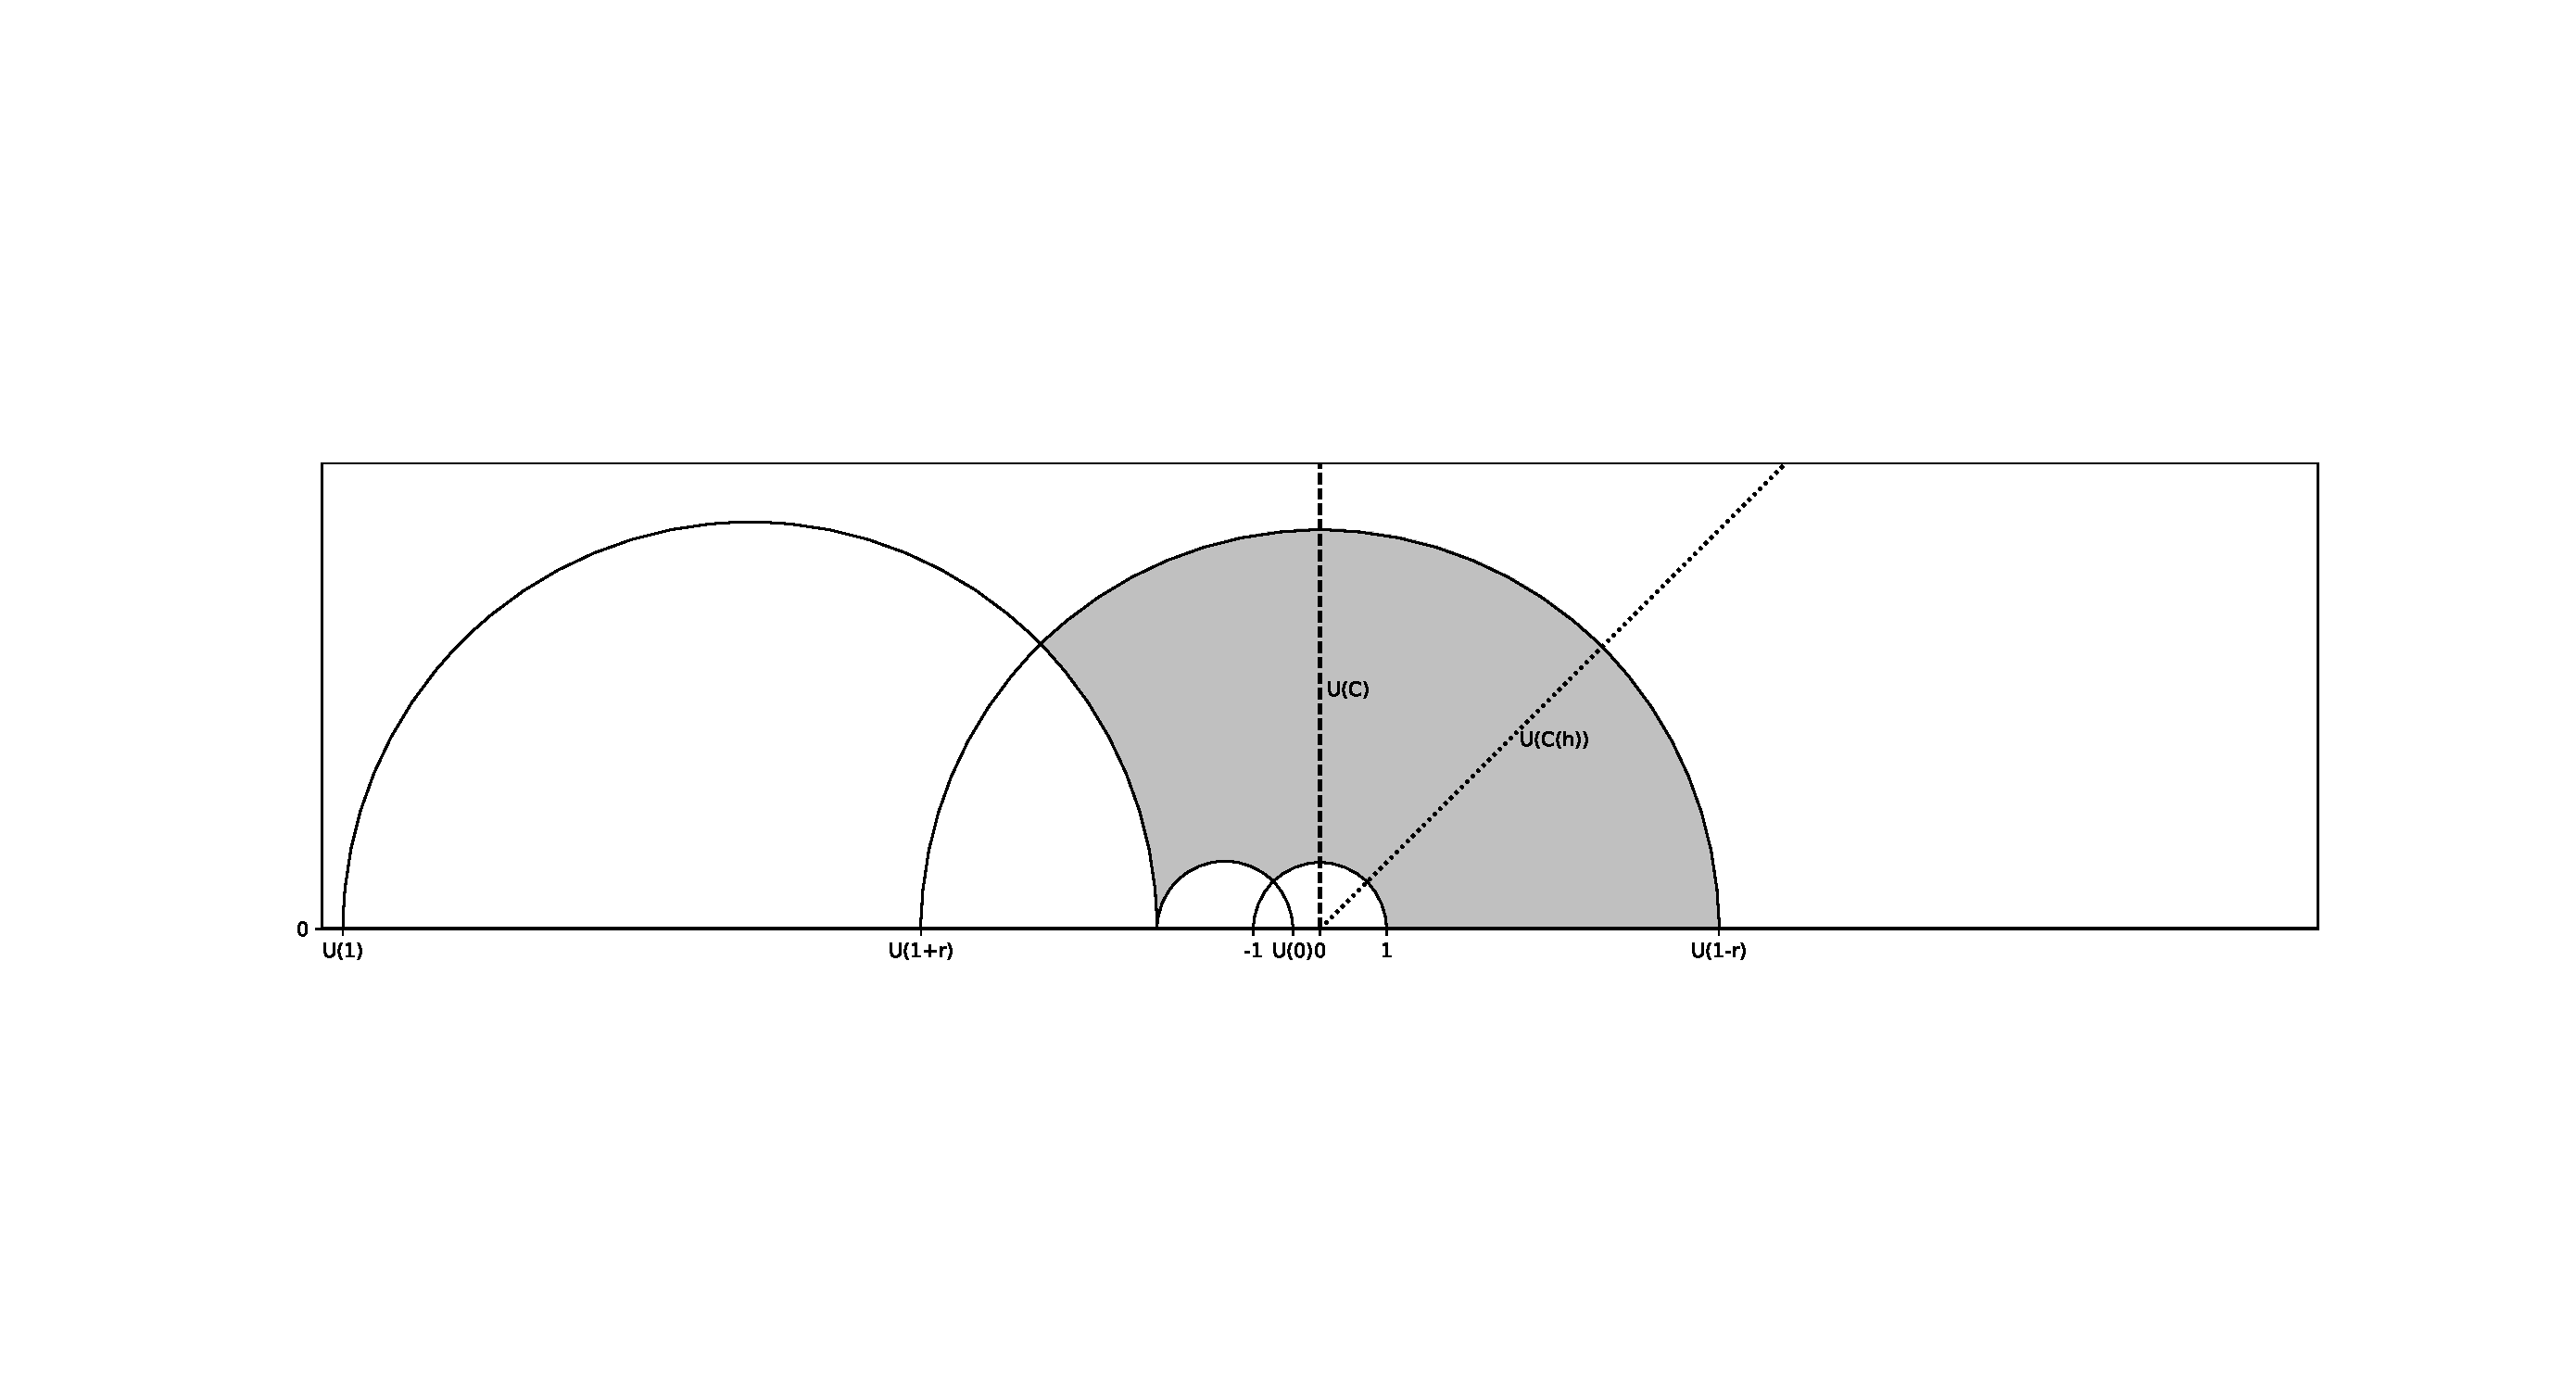
\includegraphics[trim=150 210 130 230, clip, width=\linewidth]{U_F_r.pdf}
	\caption{$U(\mathcal{F}_r)$ with $\mathcal{F}_r$ as in Figure \ref{FrWithCs}}
	\label{UFr}
\end{figure}
Note that a fundamental domain for this new action will simply be $U(\mathcal{F}_r)$, since the new group is acting on $U(\mathbb{H})$.

Let us make a few observations about the flare domain $U(\mathcal{F}_r)$.
First, note that since M\"obius transformations are conformal maps, the angle $C(h)$ makes with the real axis in the original picture is the same as the angle $U(C(h))$ makes.
So the angle parameter of our flare is the same $\alpha$ we described earlier.
Note that the scaling parameter $\kappa$ is also easily described, as
$$
\kappa = U(1-r) = \left(\frac{z_2}{r}\right)^2
$$
Since trace is conjugation invariant, we could also compute $\kappa$ by noting that
$$
\frac{1}{r} = \text{tr}(A) = \text{tr}(UAU^{-1}) = \sqrt{\kappa} + \frac{1}{\sqrt{\kappa}}
$$

\section*{Fourier Expansion in a Flare}

Let $\Gamma$ be a Fuchsian group which has a flare in its fundamental domain.
As discussed above, this implies that $\Gamma$ contains a diagonal matrix besides the identity; let's say the transformation is $z \mapsto \kappa z$ for some $\kappa > 1$.
Let $\phi$ be a Maass form on $\Gamma\backslash\mathbb{H}$, say $\Delta \phi = s(1-s)\phi$.
If we write $\phi = \phi(r, \theta)$, where $(r, \theta)$ are the usual polar coordinates, then $\phi$ is invariant under the map $r \mapsto \kappa r$.
Thus, $\phi$ has a logarithmic Fourier expansion
$$
\phi(r, \theta) = \sum_{n\in\mathbb{Z}}g_n(\theta)e\left( n\frac{\log r}{\log \kappa} \right)
$$
We would like to apply the equation $\Delta\phi = s(1-s)\phi$ to this expansion to find an explicit description of $g_n(\theta)$.
To do this, we need to know what $\Delta$ is in our new $(r, \theta)$ coordinates.
This turns out to be
\begin{equation}\label{polarL-B}
	\Delta = -\sin^2\theta\left(r^2\frac{\partial^2}{\partial r^2} + r\frac{\partial}{\partial r} + \frac{\partial^2}{\partial\theta^2}\right)
\end{equation}
Thus, by uniqueness of Fourier coefficients, $g_n(\theta)$ satisfies the differential equation
$$
\sin^2\theta\left( g_n''(\theta) + \left( \frac{2\pi in}{\log k} \right)^2g_n(\theta) \right) = s(s-1)g_n(\theta)
$$
The solution to this differential equation (which exhibits appropriate decay to ensure $\phi$ is a Maass form) is
\begin{equation}\label{solnDE}
g_n(\theta) = b_n\sqrt{\sin\theta}P^{-\nu}_{\mu_n}(\cos\theta)
\end{equation}
where
$$
\nu = s - \frac{1}{2}, ~~~ \mu_n = -\frac{1}{2} + \frac{2\pi in}{\log \kappa},
$$
and $P_\mu^{-\nu}$ is the associated Legendre function of the first kind.
(Replacing $-\nu$ with $\nu$ gives a linearly independent solution to the differential equation, but this solution does not exhibit appropriate decay at the flare).

\section*{The New Algorithm}

The way our new algorithm will differ from the previous one is to utilize the Fourier expansion at flares in addition to those at cusps.
For this explanation, let us assume that the fundamental domain for our Fuchsian group has exactly one cusp (positioned at $\infty$) and exactly one flare (perhaps after conjugation).

We denote the Fuchsian group $\Gamma$, the sought after eigenvalue $\lambda = s(1-s)$, and the eigenfunction $f$.
Let $A \in \Gamma$ be a hyperbolic matrix, then take $U \in SL(2, \mathbb{R})$ so that $UAU^{-1}$ is diagonal and a fundamental domain for the action of $U\Gamma U^{-1}$ on $U(\mathbb{H})$ contains a flare.
Finally, we let $\phi$ be the eigenfunction corresponding to $f$, where $\phi$ takes as input polar coordinates in $U(\mathbb{H})$, that is,
$$
f(z) = \phi(r(U(z)), \theta(U(z))
$$
Now recall that $f$ has an expansion at the cusp of the form
$$
f(z) = \sum_{n\in\mathbb{Z}}a_n\sqrt{y}K_\nu(2\pi|n|y)e(nx)
$$
where $K_\nu$ is the $K$-Bessel function with parameter $\nu = s - \frac{1}{2}$ and of course $z = x + iy$.
As described above, $\phi$ has an expansion at the flare of the form
$$
\phi(r, \theta) = \sum_{0 \neq n\in\mathbb{Z}}b_n\sqrt{\sin\theta}P^{-\nu}_{\mu_n}(\cos\theta)e\left( n\frac{\log r}{\log \kappa} \right)
$$
where
$$
\nu = s - \frac{1}{2}, ~~~ \mu_n = -\frac{1}{2} + \frac{2\pi in}{\log k},
$$
and $(r, \theta)$ are polar coordinates for a point in $U(\mathbb{H})$.
\\

With the notation above, we are now ready to describe the algorithm.
Hejhal's algorithm, very broadly, works like this:
\begin{itemize}
	\item We are trying to find the unknown eigenvalue $\lambda$ (equivalently, find $s$) and the unknown coefficients $a_n$ and $b_n$.
	\item To do this, we set up a grid of guesses for $s$ as well as two collections of test points $z_k$ and $w_k$.
	\item For each guess of an $s$ value and each test point, we make one or two linear equations in the unknowns $a_n$ and $b_n$.
	\item Next, we cut off the Fourier expansions to approximate the functions $f$ and $\phi$ by finite sums.
	\item So long as there are enough test points (and hence enough linear equations), we can use least squares to obtain guesses for $a_n$ and $b_n$ for $|n|$ less than our cutoff.
	\item By comparing the solution vectors $a_n, b_n$ obtained from the two sets of test points $z_k, w_k$, we can choose the $s$ value which gave the best results.
	\item We now refine our grid to look near the best $s$ value, and repeat the whole process again.
\end{itemize}

\subsection*{The Linear System}

Among all the steps described above, the one which requires the most elaboration is the setting up of linear equations given a guess $s$ and a test point $z$.
We discuss this now.

Let us fix a fundamental domain $\mathcal{F}$ for $\Gamma\backslash\mathbb{H}$ which has a cusp at $\infty$; we also assume that $U(\mathcal{F})$ is a flare domain.
Now for a test point $z \in \mathbb{H}$, we have two cases.
\\

\textit{Case 1}: $z \in \mathcal{F}$.
In this case, we obtain a linear relation by looking at the two separate expansions; namely, $f(z) = \phi(U(z))$.
After cutting off the expansions, this becomes an approximate equality:
$$
\sum_{|n| \leq M}a_n\sqrt{y}K_\nu(2\pi|n|y)e(nx) \approx
\sum_{|n| \leq M}b_n\sqrt{\sin\theta}P^{-\nu}_{\mu_n}(\cos\theta)e\left( n\frac{\log r}{\log \kappa} \right)
$$
So for each test point $z$ which falls in our fundamental domain, we get one linear equation.
\\

\textit{Case 2}: $z \notin \mathcal{F}$.
In this case, we let $z^*$ be the pullback of $z$ to $\mathcal{F}$, so $z^* \neq z$.
We will also write $(r, \theta)$ and $(r^*, \theta^*)$ for the polar coordinates of $U(z)$ and $U(z^*)$, respectively.
In this situation, we will set up one linear equation for each of the expansions of $z$.
In the first equation, we equate the cuspidal expansion at $z$ to either the cuspidal expansion at $z^*$ or the flare expansion at $(r^*, \theta^*)$.
So the first equation will be
$$
\sum_{|n| \leq M}a_n\sqrt{y}K_\nu(2\pi|n|y)e(nx) \approx
\sum_{|n| \leq M}a_n\sqrt{y^*}K_\nu(2\pi|n|y^*)e(nx^*) $$$$
\text{or} $$$$
\sum_{|n| \leq M}a_n\sqrt{y}K_\nu(2\pi|n|y)e(nx) \approx
\sum_{|n| \leq M}b_n\sqrt{\sin\theta^*}P^{-\nu}_{\mu_n}(\cos\theta^*)e\left( n\frac{\log r^*}{\log \kappa} \right)
$$
In the second equation, we equate the flare expansion at $(r, \theta)$ to either the cuspidal expansion at $z^*$ or the flare expansion at $(r^*, \theta^*)$.
So the second equation will be
$$
\sum_{|n| \leq M}b_n\sqrt{\sin\theta}P^{-\nu}_{\mu_n}(\cos\theta)e\left( n\frac{\log r}{\log \kappa} \right) \approx
\sum_{|n| \leq M}a_n\sqrt{y^*}K_\nu(2\pi|n|y^*)e(nx^*) $$$$
\text{or} $$$$
\sum_{|n| \leq M}b_n\sqrt{\sin\theta}P^{-\nu}_{\mu_n}(\cos\theta)e\left( n\frac{\log r}{\log \kappa} \right) \approx
\sum_{|n| \leq M}b_n\sqrt{\sin\theta^*}P^{-\nu}_{\mu_n}(\cos\theta^*)e\left( n\frac{\log r^*}{\log \kappa} \right)
$$
Note: typically, we will make a choice for each test point whether to use the cuspidal expansion or the flare expansion at its pullback.
This choice will not be arbitrary, as seen in the discussion on ``admissible points'' below.

\subsection*{Admissibility of Test Points}

Recall that each expansion is associated with either a cusp or a flare.
It turns out that the closer a point is to a cusp or flare, the better that expansion converges.
In a moment, we will make this statement more precise, but first let us say what this means for our algorithm.
\\

Fix a height $y_0 > 0$ and an angle $0 < \theta_0 < \pi$.
We will say a point $z \in \mathbb{H}$ is \textit{admissible with respect to the cuspidal expansion} if $\text{Im}(z) \geq y_0$.
This definition, of course, is dependent on the parameter $y_0$.
Similarly, if a point $z \in \mathbb{H}$ has $\arg z \leq \theta_0$, then we say $z$ is \textit{admissible with respect to the flare expansion}.
Again, keep in mind that this definition depends on the parameter $\theta_0$.
To justify these definitions, see the discussion on asymptotics of the Fourier coefficients below.

To make sure our cutoff of the Fourier expansions is appropriate, we will only use admissible points in the linear system.
For example, if a test point already lies in the fundamental domain $\mathcal{F}$, then we will require it to be admissible with respect to both expansions simultaneously (since the linear equation we set up for such points utilizes both expansions).
Note that this explains how we will choose which expansion to use for the pullback points.
If a pullback is admissible with respect to both expansions, then it is immaterial which expansion we choose.

\subsection*{Asymptotics in the Cuspidal Expansion}

\textbf{THIS IS WRONG! COPY OVER ARGUMENT FROM FLAREASYMPTOTICS.PDF ONCE THAT'S FINISHED.}

For the cuspidal expansions, recall that the $n^{th}$ Fourier coefficient is
\begin{equation}\label{cuspCoeff}
a_n\sqrt{y}K_\nu(2\pi|n|y)
\end{equation}
It can be shown that $K_\nu(Y)$ decays exponentially as $y \rightarrow \infty$.
On the other hand, note that
$$
a_n\sqrt{y}K_\nu(2\pi|n|y) = \int_{0}^{1}f(x + iy)e(-nx)dx
$$
where we write $f(z)$ for the Maass form.
It can be shown that $f$ is bounded in a neighborhood of the cusp and that it goes to $0$ as $z$ approaches a flare.
Thus, $|f(z)|$ is bounded on $\mathbb{H}$.
Hence,
$$
|a_n\sqrt{y}K_\nu(2\pi|n|y)| \leq \int_{0}^{1}|f(z)|dx \leq C
$$
for some $C > 0$.
Since this estimate is independent of $y$, we may choose $y = 1/n$ to remove the dependence of the estimate on the $K$-Bessel function.
This shows that
$$
a_n = O(\sqrt{n})
$$
(Note: it is possible to show the stronger result that $a_n = O(1)$, but this requires a more involved proof).
Hence, the entire Fourier coefficient (\ref{cuspCoeff}) decays exponentially with $n$.
In fact, we expect the Fourier expansions to converge rapidly as soon as $n \approx 1/y$.
This shows that larger $y$ require less terms in the Fourier expansion to give a good approximation, hence justifying our definition of admissible points with respect to the cuspidal expansion.

\subsection*{Asymptotics in the Flare Expansion}

\textbf{THIS IS WRONG! COPY OVER ARGUMENT FROM FLAREASYMPTOTICS.PDF ONCE THAT'S FINISHED.}
\\

For the flare expansions, recall that the $n^{th}$ Fourier coefficient is
$$
b_n\sqrt{\sin\theta}P^{-\nu}_{\mu_n}(\cos\theta)
$$
where $\nu = s - \frac{1}{2}$, $\mu_n = -\frac{1}{2} + \frac{2\pi in}{\log\kappa}$, and $0 < \theta < \pi$.
To replicate the analysis from the cuspidal expansion, we require some asymptotics on the Legendre $P$ function.

\textbf{Figure out why small $\theta$ is a good choice!}

We make use of the Digital Library of Mathematical Functions (DLMF) to get asymptotics on the Legendre $P$ function.
We start with equation 14.15(iii) in the DLMF:
$$
P_\mu^{-\nu}(\cos\theta) = \frac{1}{\mu^\nu}\sqrt{\frac{\theta}{\sin\theta}}\left( J_\nu((\mu+1/2)\theta) + O\left( \frac{1}{\mu} \right)\text{env}J_\nu((\mu+1/2)\theta) \right)
$$
where $J_\nu$ is the $J$-Bessel function and $\text{env}J_\nu$ is defined in the DLMF.
This statement holds uniformly for $\theta \in (0, \pi - \delta]$ as $|\mu| \rightarrow \infty$ for fixed $\nu \geq 0$.
Since we are interested in the behavior as $|\mu|$ gets large, we will content ourselves with the statement
$$
P_\mu^{-\nu}(\cos\theta) \sim \frac{1}{\mu^\nu}\sqrt{\frac{\theta}{\sin\theta}}J_\nu((\mu+1/2)\theta)
$$
as $|\mu| \rightarrow \infty$.

Next, we need asymptotics for the $J$-Bessel function.
Equation 10.7(ii) in the DLMF states that
$$
J_\nu(z) = \sqrt{\frac{2}{\pi z}}\left( \cos\left(z - \frac{\nu\pi}{2} - \frac{\pi}{4}\right) + e^{|\text{Im}(z)|}o(1) \right)
$$
for fixed $\nu$ as $|z| \rightarrow \infty$.
In particular, if $\text{Im}(z)$ is becoming large, we have that
$$
J_\nu(x + iy) \sim y^{-1/2}e^{|y|}
$$
as $y \rightarrow \pm\infty$.

Putting these estimates together, we expect for
$$
\mu_n := -\frac{1}{2} + \frac{2\pi in}{\log\kappa}
$$
to have
\begin{equation}\label{legPAsymptotic}
P_{\mu_n}^{-\nu}(\cos\theta) \sim (\sin\theta)^{-1/2}|n|^{-\nu-1/2}e^{2\pi|n|\theta/\log\kappa}
\end{equation}
as $|n| \rightarrow \infty$.
Note that this asymptotic holds \textit{uniformly for} $\theta \in (0, \pi - \delta]$.

We now return to the analysis of the Fourier coefficient.
As before, we use the fact that a Maass form $\phi(r, \theta)$ is bounded on $\mathbb{H}$ to conclude that
$$
|b_n\sqrt{\sin\theta}P_{\mu_n}^{-\nu}(\cos\theta)| =
\left| \int_{1}^{\kappa}\phi(r, \theta)e\left( -n\frac{\log r}{\log\kappa} \right)\frac{dr}{r}\right| \leq \int_{1}^{\kappa}|\phi(r, \theta)|\frac{dr}{r} \leq C
$$
Applying the asymptotic (\ref{legPAsymptotic}), we have that
$$
|b_n| \leq C'|n|^{\nu+1/2}e^{-2\pi|n|\theta/\log\kappa}
$$
\textbf{Think about the implications of this.}

\section*{Verification of Formula (\ref{polarL-B})}

In the upper half plane model of hyperbolic space, the Laplace-Beltrami operator is
$$
\Delta = -y^2\left( \frac{\partial^2}{\partial x^2} + \frac{\partial^2}{\partial y^2} \right)
$$
where $z = x + iy \in \mathbb{H}$.
\\

Next, we wish to rewrite the Laplace-Beltrami operator in $(r, \theta)$ polar coordinates.
What exactly does this mean?
If $f : \mathbb{H} \rightarrow \mathbb{C}$ is a function in $(x, y)$ coordinates and $g : \mathbb{H} \rightarrow \mathbb{C}$ is a function in $(r, \theta)$ coordinates, then we think of $f$ and $g$ as the same function if
$$
f(x, y) = g(r(x, y), \theta(x, y)) ~~\forall~x + iy \in \mathbb{H}
$$
where $(r(x, y), \theta(x, y))$ describes the same point in $\mathbb{H}$ as $x + iy$.
Now, the functions we are interested in are those which are differentiable in the $\mathbb{R}^2$ sense.
So by applying the chain rule for functions from $\mathbb{R}^2$ to $\mathbb{R}^2$, we conclude that
$$
\frac{\partial^2f}{\partial x^2} =
\frac{\partial^2r}{\partial x^2}\frac{\partial g}{\partial r} +
\frac{\partial^2\theta}{\partial x^2}\frac{\partial g}{\partial\theta} +
\left(\frac{\partial r}{\partial x}\right)^2\frac{\partial^2 g}{\partial r^2} +
2\frac{\partial r}{\partial x}\frac{\partial\theta}{\partial x}\frac{\partial^2 g}{\partial r\partial\theta} +
\left(\frac{\partial\theta}{\partial x}\right)^2\frac{\partial^2 g}{\partial\theta^2} $$$$
\frac{\partial^2f}{\partial y^2} =
\frac{\partial^2 r}{\partial y^2}\frac{\partial g}{\partial r} +
\frac{\partial^2\theta}{\partial y^2}\frac{\partial g}{\partial\theta} +
\left(\frac{\partial r}{\partial y}\right)^2\frac{\partial^2 g}{\partial r^2} +
2\frac{\partial r}{\partial y}\frac{\partial\theta}{\partial y}\frac{\partial^2 g}{\partial r\partial\theta} +
\left(\frac{\partial\theta}{\partial y}\right)^2\frac{\partial^2 g}{\partial\theta^2}
$$
I used python to compute these; one finds that
$$
\frac{\partial^2f}{\partial x^2} + \frac{\partial^2f}{\partial y^2} =
\frac{\partial^2 g}{\partial r^2} + \frac{1}{r}\frac{\partial g}{\partial r} + \frac{1}{r^2}\frac{\partial^2g}{\partial\theta^2}
$$
This verifies formula (\ref{polarL-B}).

\section*{Verification of Formula (\ref{solnDE})}

I ``verified'' this numerically using python.
See verifyFormulas.py for details.
	
\end{document}